\documentclass[a4paper]{article}
\usepackage{amsfonts}
\usepackage{amsmath}
\usepackage{amssymb}
\usepackage{graphicx}     

\begin{document}
  
\noindent \large Auteur: CouldBeMathijs \\
\noindent \large Studierichting: Informatica\\
\noindent \large Oefeningenreeks 3H nr. 14.3\\

\medskip

\normalsize

\begin{center}
 Legende:
\end{center}
\begin{figure}[h]
    \centering
    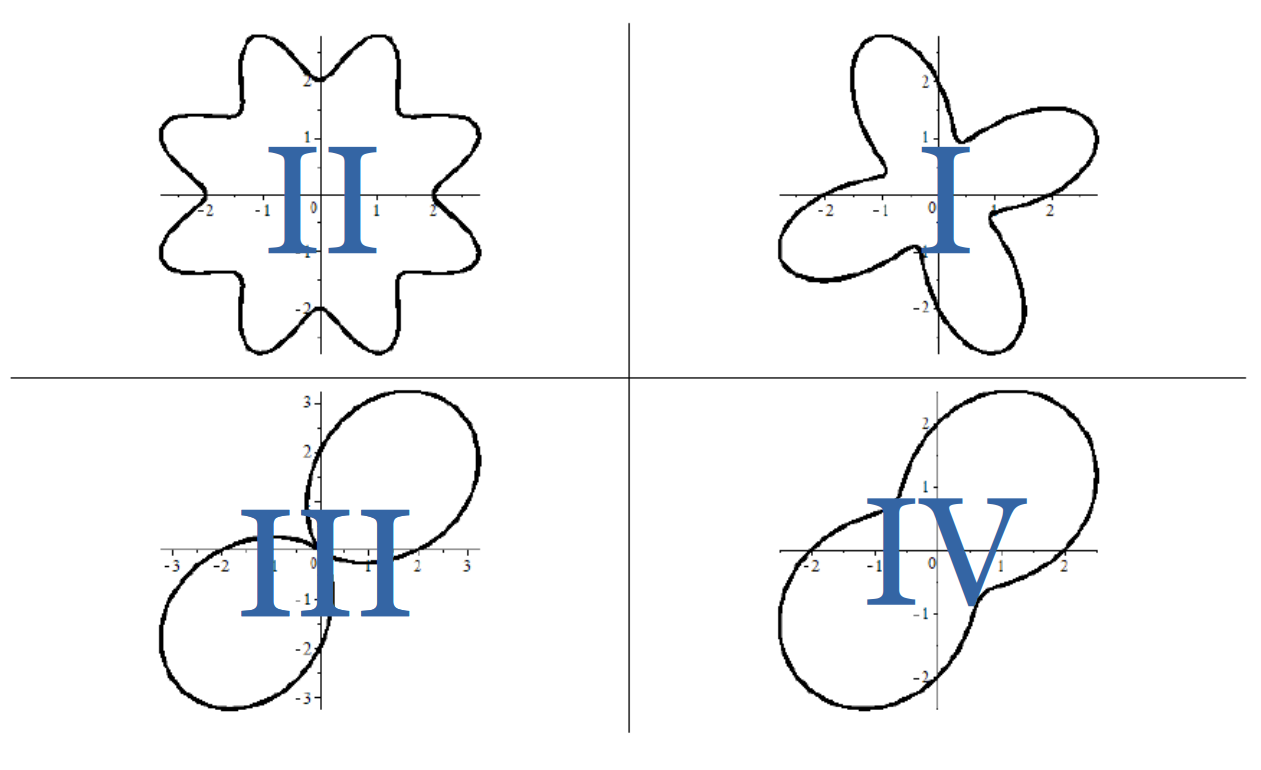
\includegraphics[width=5cm]{3H-14.3-could.be.mathijs.INF.png}
\end{figure}

A) $r=2+\sin 4\theta$\\

Beschouw het bereik van $r$: $[2-1, 2+1] = [1, 3]$: enkel \textbf{I} voldoet\\

B) $r = 2 + 2\sin 2\theta$\\

Bereik van $r$: $[2-2, 2+2] = [0, 4]$: enkel \textbf{III} gaat door de oorsprong\\

C) $r= 2 + \sin 2 \theta$\\

Functievoorscrift lijkt op (B) met minder grote verandering van $r$: \textbf{IV}\\

D) $r=2\sin^24\theta$\\

Enkel \textbf{II} blijft nog over


\begin{thebibliography}{999}
%\bibitem{a} Referentie
\end{thebibliography}
\end{document} 
